% begin module improper-integral-comparison
\begin{frame}
\frametitle{A Comparison Test for Improper Integrals}
Sometimes it's impossible to find the exact value of an integral, but we still want to know if it's convergent or divergent.  For such cases, we can sometimes use this theorem.
\begin{theorem}[Comparison Theorem]
Suppose $f$ and $g$ are continuous and $f(x) \geq g(x) \geq 0$ for $x \geq a$.
\begin{enumerate}
\item  If $\int_a^\infty f(x) \diff x$ is convergent, then $\int_a^\infty g(x)\diff x$ is convergent.
\item  If $\int_a^\infty g(x) \diff x$ is divergent, then $\int_a^\infty f(x)\diff x$ is divergent.
\end{enumerate}
\end{theorem}
\begin{columns}[c]
\column{.4\textwidth}
\ 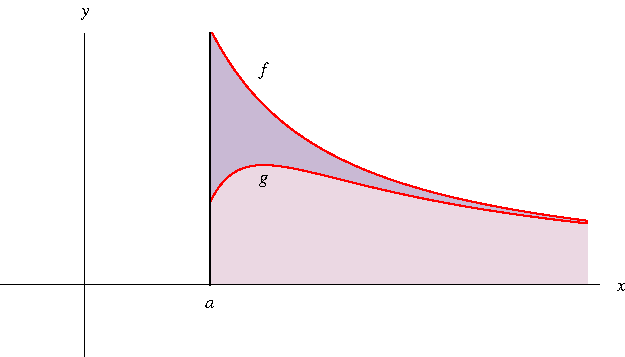
\includegraphics[height=3cm]{improper-integrals/pictures/08-08-comptest.pdf}%
\column{.6\textwidth}
\uncover<2->{%
A similar theorem holds for Type II improper integrals.
}%
\end{columns}
\end{frame}
% end module improper-integral-comparison
